\chapter{Inleiding}
De hedendaagse meest gebruikte database management systemen (DBMS's) zijn relationele of NoSQL DBMS's \cite{dbengine-ranking}. De NoSQL systemen bestaan uit een waaier van systemen met verschillen in datamodel, performantie, beschikbaarheid of consistentie. 
Het CAP theorema van Erik Brewer\cite{Brewer:2000:TRD:343477.343502} stelt dat elk gedistribueerd dataopslag niet tegelijk onmiddellijke consistentie, hoge beschikbaarheid en partitie tolerant kan zijn. Elk DBMS maakt zijn eigen keuze en afweging tussen de verschillende garanties en eigenschappen die het levert. 

Deze thesis beschrijft een testmethode om DBMS's te vergelijken op basis van de consistentie- en beschikbaarheidsgaranties. De methode onderzoekt het gedrag van het volledige DBMS bij het in- en uitschakelen van een server of netwerkverbinding. Daarnaast wordt bestudeerd hoe de data van een schrijfbewerking zichtbaar wordt voor gelijktijdige leesbewerkingen. Deze testen worden gebruikt om het theoretische beschreven gedrag te vergelijken met de praktijk. Daarnaast kunnen de verschillen tussen DBMS's vergeleken worden.

Drie consistentie en partitie tolerante systemen worden ontworpen aan de testmethode: HBase en MongoDB zijn NoSQL systemen, PgPool-II (PostgreSQL) is een relationeel systeem. Uit de resultaten blijkt dat PgPool-II op een andere wijze de beschikbaarheid van de verschillende systemen registreert dan de 2 andere systemen. HBase en MongoDB behandelen verschillend gelijktijdige lees- en schrijfbewerking op dezelfde data. HBase zal leesbewerkingen uitstellen tot een volledige voltooiing van de schrijfbewerking, MongoDB zal de leesbewerkingen al nieuwe data laten lezen voor het volledig voltooien van de schrijfbewerking. 

De volgende sectie behandelt een bespreking van relationele en NoSQL DBMS's, gevolgd door een overzicht van de testmethodes voor de thesis waaruit zal blijken dat er een afwezigheid is van testmethodes naar consistentie en beschikbaarheid. Daarna zullen de doelstellingen en bijdrage van de thesis geformuleerd worden. Tenslotte wordt een overzicht gegeven van de rest van de thesis. 


%
%De NoSQL databases zijn een nieuwe generatie van systemen, de NoSQL beweging is gestart in 2000 en staat voor '\textit{Not only SQL}'. Deze systemen zijn er gekomen als op de globalisering van de computer systemen. Met een geografische spreiding van de verschillende datacentra konden de RDBMS niet om?. Dit leidde tot de nood voor meer flexibele databases, een lagere complexiteit, hogere doorvoer van data, horizontale schaalbaarheid en het draaien op commodity hardware. NoSQL DBMS proberen hieraan te voldoen met voorbeelden als Google BigTable, Amazon Dynamo, HBase, MongoDB, ... \cite{Strauch.NoSQL} 
%
%In de volgende sectie zullen beide systemen in meer detail aanbod komen, waarna de huidige staat voor het kwantitatief vergelijken van de systemen aan bod. Tenslotte zullen de doelstellingen en de bijdragen van de thesis toegelicht worden. 

\section{Relationele en NoSQL DBMS's} 
Zoals voordien vermeldt, zijn de populaire DBMS's momenteel de relationele en NoSQL systemen. In deze sectie zullen beide categorieën besproken worden, eerst komt het relationele DBMS aan bod, gevolgd door NoSQL. 

\subsection{Relationele database}
Het RDBMS is gebaseerd op het relationele model voor het structureren van de data in een database. Dit model is uitgebreid bespoken in het artikel van E. Codd \cite{codd1970relational}. Voorbeelden van hedendaagse populaire relationele DBMS's (RDBMS's) zijn Oracle, MySQL en PostgreSQL. 

Het relationele model vertrekt van theoretische wiskundige principes zoals de set-theorie en de eerste-orde predicaten logica. Het model organiseert de data in tabellen en legt relaties tussen de tabellen. De tabel heeft kolommen die verschillende velden voorstellen waarbij elke rij een collectie van gerelateerde datawaardes is. De relaties tussen de verschillende tabellen tonen hoe deze bij elkaar horen. Een belangrijke eigenschap is dat de tabellen en relaties genormaliseerd worden, hiermee wordt redundante informatie verwijderd. Dit zorgt voor een hogere data integriteit en een vermindering in data anomalieën die kunnen optreden bij een update.\cite{Elmasri:2010:FDS:1855347} \\
De normalisatie kan geïllustreerd worden met het korte voorbeeld van figuur \ref{fig:Relationeel-Model-Normalisatie}: de professor voor een vak zal bij elke student hetzelfde zijn, het veranderen van een professor voor een vak zou in het eerste geval een update van alle ingeschreven studenten inhouden. In het tweede geval is dit maar de aanpassing van een enkel record, dezelfde gedachtegang is toepasbaar op de student. \\
Interactie met de RDBMS gebeurt op basis van SQL (Structured Query Language), een taal gebaseerd op de relationele logica. SQL geeft uitgebreide query mogelijkheden aan de gebruiker van de software.   
\begin{figure}[ht!]
\centering
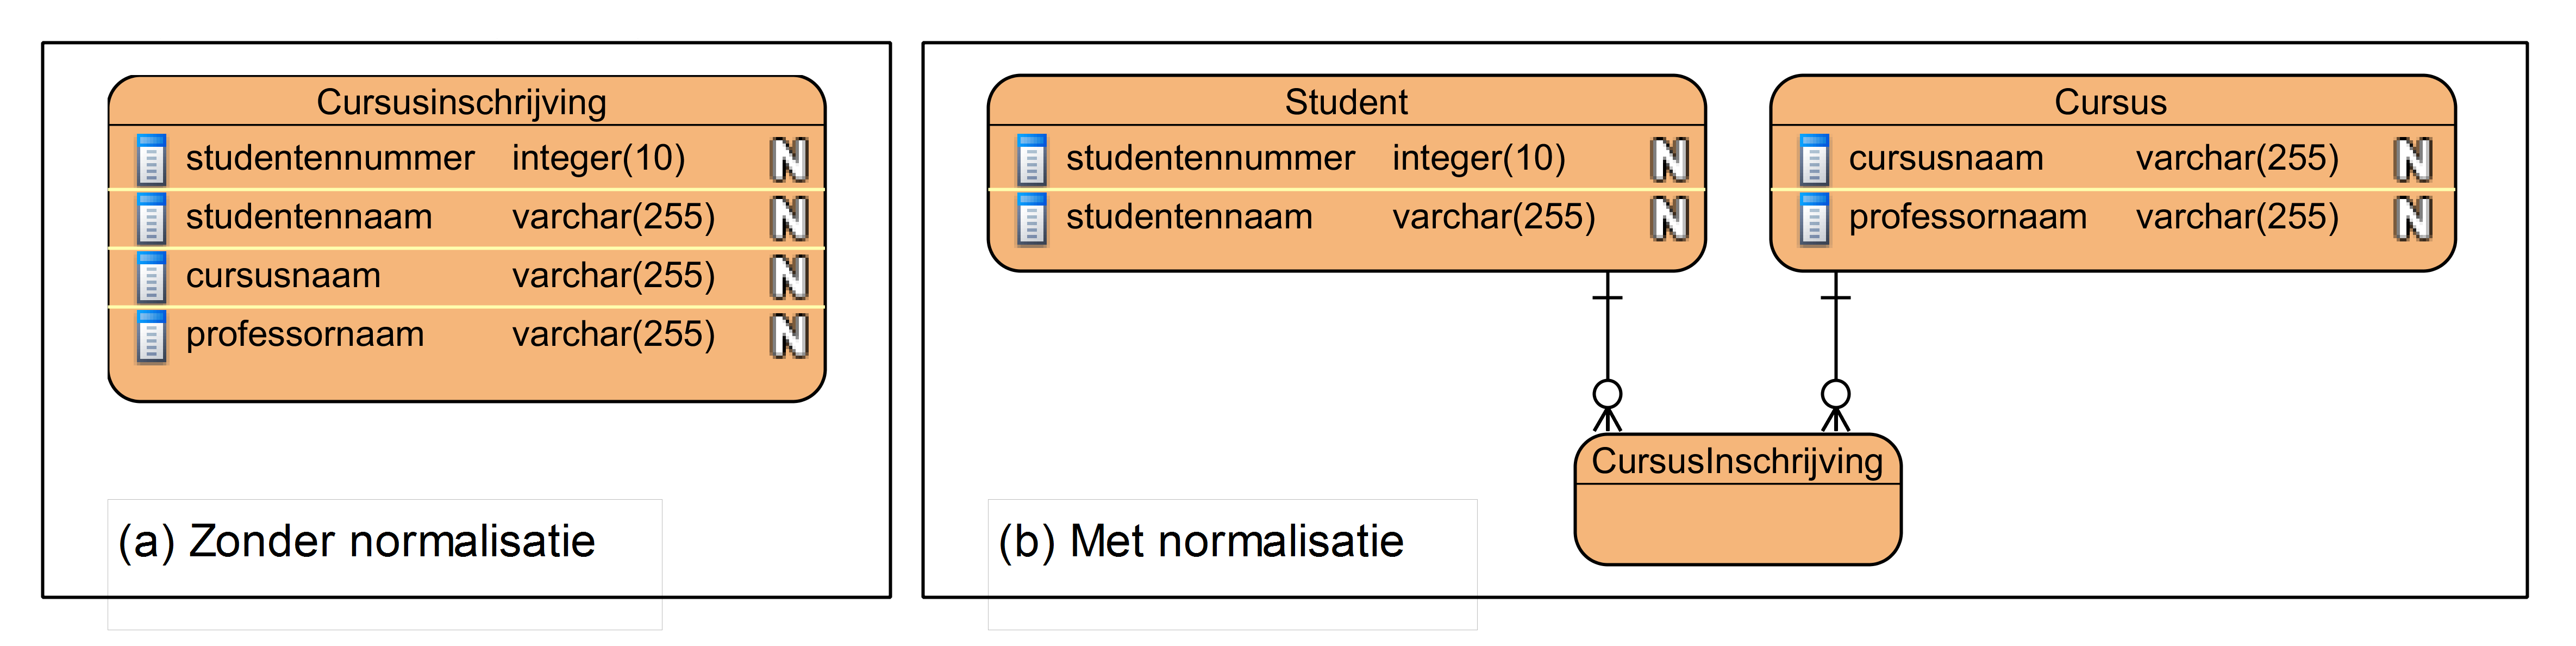
\includegraphics[width=\linewidth]{img/Relationeel-Model-Normalisatie.png}
\caption[Relationeel datamodel (a) zonder en (b) met normalisatie]{Relationeel datamodel (a) zonder en (b) met normalisatie}
\label{fig:Relationeel-Model-Normalisatie}
\end{figure}

Een belangrijk concept in een relationele database is ACID, welk voor betrouwbare en robuuste transacties zorgt. 

\paragraph{Atomair (\underline{A}tomicity)} Of een database transactie moet volledig uitgevoerd worden, of er heeft geen enkele bewerking plaatsgevonden. 

\paragraph{Consistent (\underline{C}onsistency)} Een transactie behoudt consistentie als de volledige uitvoering van de transactie de database van een consistente staat naar een andere consistentie staat brengt. Een consistente staat is een staat die ervoor zorgt dat waardes van een instantie consistent zijn met de andere waarden in dezelfde staat. Een voorbeeld is het overschrijven van \euro{50} van persoon A naar B, op het einde moet de totale som nog steeds gelijk zijn, A \euro{50} minder en B \euro{50} meer. Een inconsistente staat zou zijn dat enkel A \euro{50} minder heeft, maar B nog steeds evenveel geld. 

\paragraph{Geïsoleerd (\underline{I}solation)} Een transactie moet uitgevoerd worden alsof ze volledig voor of na andere transacties heeft plaatsgevonden. 

\paragraph{Duurzaam (\underline{D}urability)} Een voltooide transactie kan later niet ongedaan gemaakt worden.

Deze verschillende concepten bieden de garanties welke de gebruiker kan gebruiken voor zijn systeem. Daartegenover staat wel dat dit de complexiteit van de RDBMS groeit, ook indien dit voor bepaalde toepassingen misschien niet nodig is. Een moeilijkheid is het schalen van het systeem bij een groter wordende dataset; door het toepassen van normalisatie dient er bij een enkele query data van verschillende tabellen gecombineerd te worden. Dit zorgt ervoor dat er in eerste instantie verticaal geschaald zal worden, het gebruiken van krachtigere hardware. Het toevoegen van extra servers, horizontaal schalen, is in veel gevallen slechts beperkt ondersteund. 


\subsection{NoSQL database\cite{Strauch.NoSQL}}\label{sec:eventualconsistency}
NoSQL DBMS zijn ontstaan door groei en globalisering van de computersystemen en de bijhorende databases. Een RDBMS is gebouwd met een 'one size fits all'-gedachte, maar deze systemen veroorzaken hiermee complexiteit die voor bepaalde toepassingen niet nodig is. NoSQL systemen bestaan in verschillende variëteiten, elk met hun eigen eigenschappen en toepassingsgebied om zo de complexiteit te verminderen. Tussen deze verschillen is er een rode draad te vinden in vergelijking met een RDBMS:
\begin{itemize}
	\item \textbf{Lagere complexiteit}: NoSQL systemen bieden minder opties en garanties dan de RDBMS, bepaalde applicaties hebben enkel nood aan een deel van de garanties. Bijvoorbeeld in een sociale netwerk moet een post niet onmiddellijk beschikbaar zijn voor al de vrienden van een persoon, maar mag dit even duren.
	\item \textbf{Hogere doorvoer}: Talrijke NoSQL systemen bieden een hogere doorvoer van data aan. In veel gevallen is dit een gevolg van de lagere complexiteit of door de hulp van andere bewerkingen zoals MapReduce \cite{dean2008mapreduce}.
	
	\item \textbf{Horizontale schaalbaarheid en werkend op commodity hardware}: Waar grote RDBMS's werken met dure high-end systemen, was het bedoeling van NoSQL databases ondersteuning te bieden aan een veelvoud van geclusterde eenvoudige machines (commodity hardware). \\
	Horizontale schaalbaarheid staat voor het toevoegen extra machines aan een systeem voor extra resources, in tegenstelling tot verticale schaalbaarheid waar een krachtigere machine wordt gebruikt voor de opschaling. De horizontale opschaling wordt tot uitvoering gebracht door de data van een enkele database of tabel te verspreiden over verschillende machines die elk maar voor een deel van de data verantwoordelijk zijn en moeten opslaan.\\
	NoSQL systemen combineren deze twee elementen en bieden hierdoor een schaalbaar systeem aan met basis componenten.
	\item \textbf{Datamodel dichter bij objecten}: De meeste NoSQL systemen zijn zodanig ontworpen dat deze de vertaling van objecten naar opslag eenvoudiger maken t.o.v. RDBMS's. RDBMS zijn ontworpen voor het ontstaan van object georiënteerde programmeertalen en heeft nood aan de vertaling van een object naar een databasestructuur. Bij het ontwerp van NoSQL systemen werd er hiermee onmiddellijk rekening gehouden.  
\end{itemize}  \noindent
Deze verschillende argumenten leiden vervolgens tot BASE, een tegenreactie op ACID. \noindent 
\begin{itemize}
 \item Basis beschikbaarheid (\textbf{B}asically \textbf{A}vailability): het DBMS biedt lees- en schrijfacties aan bij het falen van één of meerdere falende instanties. De ondersteuning is afhankelijk van systeem tot systeem samen met de configuratie. 
 \item \textbf{S}oft State: De data moet op een bepaald moment niet volledig consistent zijn. 
 \item Uiteindelijke consistentie (\textbf{E}ventual Consistency): De database zal na enige tijd in een consistente status uitkomen, het is mogelijk dat oudere data tijdelijk leesbaar is. Eventuele consistentie kan op zijn beurt opnieuw onderverdeeld worden in 4 categorieën \cite[slide 16]{lipcon2009design}:
 	\begin{itemize}
 		\item \textit{Read your own writes} consistentie: Ongeachte van de server waarop een gebruiker leest, zal hij zijn schrijfactie onmiddellijk correct lezen. 
 		\item \textit{Session} consistentie: De gebruiker zal zijn schrijfactie onmiddellijk kunnen lezen binnen dezelfde sessie, een sessie is hierdoor meestal gelimiteerd tot een enkele database server. 
 		\item \textit{Casual} consistentie: Als een gebruiker versie X leest en vervolgens versie Y van een verschillend dataelement schrijft, zal elke gebruiker die versie Y leest ook versie X lezen.
 		\item \textit{Monotonic Read} consistentie: Dit levert monotone tijdsgaranties dat een gebruiker enkel recentere data versies in de toekomst zal lezen. 
 	\end{itemize}
\end{itemize}
De BASE eigenschappen kunnen gekoppeld worden aan het CAP theorema van Erik Brewer\cite{Brewer:2000:TRD:343477.343502}. CAP zegt dat een gedistribueerd systeem maar twee van de drie CAP elementen kan ondersteunen: consistentie, beschikbaarheid en partitie tolerantie. De beschikbaarheid betekent dat bij het falen van een instantie er nog steeds schrijfbewerkingen mogelijk zijn. Bij partitie tolerantie kan het systeem overweg met het opgesplitst zijn van instantie door een niet werkende netwerk verbinding. De definitie van consistentie is hier anders als bij ACID: bij CAP is er sprake van consistentie als het DBMS zich gedraagt alsof er maar één dataopslag is.

\subsubsection{Classificatie van NoSQL systemen}
Er zijn vele NoSQL systemen ontworpen gedurende de laatste jaren, elk met hun eigen variëteit, functionaliteit en populariteit. Er bestaan verschillende manieren om de systemen te classificeren, maar één van de meest gebruikte doet dit op basis de data modellering. Een korte vergelijking op basis van deze bevindt zich in tabel \ref{table:selectie-classificatie}.  

\begin{table}[!h]
	\resizebox{\textwidth}{!} {
		\begin{tabular}{l l l l l l}
			\textbf{Soort} & \textbf{Performantie} & \textbf{Schaalbaarheid} & 			\textbf{Flexibiliteit} & \textbf{Complexiteit} & \textbf{Functionaliteit} \\ \hline
			Column & hoog & hoog & gematigd & laag & minimaal \\
			Document & hoog & variabel(hoog) & hoog & laag & variabel (laag) \\
			Graph & variabel & variabel & hoog & hoog & graph theory \\
			Key-Value & hoog & hoog & hoog & geen & variabel (geen) \\
		\end{tabular}
	}
	\caption{Classificatie en categorisatie van NoSQL DBMS's door Scofield en Popescu. \cite{categorizatie-sco10} \cite{categorizatie-pop10b} }
	\label{table:selectie-classificatie}
\end{table} 

\paragraph{Column Model}In een column-gebaseerd systeem wordt de data opgeslagen per kolom in plaats van de traditionele manier, per rij. Deze aanpak werd in eerste instantie gedaan voor analyse van business intelligentie. Het systeem is geïnspireerd door de paper van Google’s Bigtable \cite{chang2008bigtable}. \cite{Strauch.NoSQL}

\paragraph{Document Model} Document systemen zijn volgens vele de volgende stap in key-value systemen, waar deze complexere structuren toe laten, dit door middel van meerdere key/value paren per element. \cite{Strauch.NoSQL} \\
Een document moet geen vaste structuur hebben maar elk document op zich kan verschillende velden hebben, dit kan bijvoorbeeld toegepast worden bij boeken. Waar een bepaald boek een recept is, kan een ander een deel zijn van een trilogie. Bij het eerste kan de kooktijd opgeslagen worden en bij de tweede een referentie naar de andere boeken. \cite{Strauch.NoSQL}

\paragraph{Graph Model} In een grafen model, wordt de data voorgesteld en opslagen volgens de grafen theorie: knopen, lijnen en eigenschappen op de knopen en lijnen. \cite{bollacker2008freebase}.   

\paragraph{Key-Value Model} Key-Value systemen hebben een heel eenvoudig data model, data kan opgeslagen, opgevraagd en verwijderd worden op basis van een key. De informatie die in de database zit, is de waarde voor die key. \\
Met dit eenvoudig model en functionaliteit die weinig complexiteit introduceren, kan er gestreefd worden naar een hoge performantie, schaalbaarheid en flexibiliteit. \cite{Strauch.NoSQL}


\subsection{Bespreking van verschillende DBMS's}
Voorbeeldsystemen uit de relationele systemen en 3 categorieën van NoSQL komen verder aan bod. Er is gekozen om de Graph NoSQL DBMS's niet te bespreken. Graph NoSQL DBMS's zijn bedoeld voor de opslag van data van grafen. Deze is significant verschillend van de andere categorieën en hierdoor niet opgenomen. 
 
\begin{itemize}
\item Column NoSQL DBMS's: Cassandra, HBase
\item Document NoSQL DBMS's: Apache CoucheDB, MongoDB
\item Key-Value NoSQL DBMS's: LightCloud (Tokyo), MemCache, Redis, Riak, Project Voldemort
\item Relationele DBMS's: MySQL, Pgpool-II (PostgreSQL)
\end{itemize}

Deze keuze van deze systemen is gebaseerd op de paper van Christophe Strauch \cite{Strauch.NoSQL}. Een korte bespreking van de verschillende systemen kan gevonden worden in bijlage \ref{sec:BesprekingDBMS}.


\section{Vergelijking van DBMS's naar performantie en CAP}
Bij de ontwikkeling van verschillende systemen is er een keuze naar welk DBMS er kozen wordt. De systemen verschillen en hebben elk hun eigen toepassingsgebied. Zoals besproken hierboven kan een opsplitsing naar het datamodel gemaakt worden, of in meer detail naar de ondersteunde database bewerkingen. 

Maar de systemen maken ook keuzes uit performantie en CAP theorema, deze keuzes hebben hun invloed op de prestaties en het gedrag voor de gebruikers. In deze sectie zal er gekeken worden welke methodes er reeds beschikbaar zijn voor het analytisch vergelijken van de performantie, consistentie en beschikbaarheid op basis van het gedrag in de praktijk. Daarnaast worden al mogelijke resultaten kort besproken.   

\subsection{Performantie benchmarking}
Voor de vergelijking van de performantie van verschillende DBMS's bestaan er reeds enkele tools en studies. Een blogpost van A. Popescu \cite{PopescuBenchmarkOverview} geeft een overzicht van verschillende benchmarking tools. 

Vele DBMS's hebben \textbf{interne benchmarking tools}, waarmee de database op verschillende configuraties kunnen getest en vergeleken worden. Deze resultaten zijn nuttig na het kiezen van een DBMS. Het systeem kan getest worden met variërende parameters en kan helpen met het uitzoeken wat de bottleneck is van een bepaald systeem. Een voorbeeld hiervan is mongoperf\footnote{\url{http://docs.mongodb.org/manual/reference/program/mongoperf/}} voor MongoDB. 

Andere studies focussen op het testen van verschillende systemen en daarbij kunnen verschillende doelstellingen zijn: het ontwikkelen van een breed toepasbare tool, het testen van een grote verscheidenheid van DBMS's of een specifieke categorie van systemen, beide met een focus op het publiceren van de resultaten. Elke van deze studies brengt nieuwe kennis van de systemen maar heeft ook zijn beperkingen. Het totaal pakket kan een gebruiker de informatie geven om een beter gefundeerde keuze te maken. 

Een eerste categorie van deze externe tools is het \textbf{ontwikkelen van een tool} voor verschillende systemen. Dit heeft als grote voordeel dat andere gebruikers nadien de testen opnieuw kunnen uitvoeren met de systemen in hun configuratie. Het is namelijk niet gegarandeerd dat het resultaat van een jaar geleden overeenstemmend is met de nieuwste versie.
Het grootste nadeel is de testen die kunnen uitgevoerd worden, er is een grote variëteit aan systemen elk met hun eigen datastructuur en query mogelijkheden. De tool moet dus een gemeenschappelijke subset zoeken en enkel dit soort queries kunnen getest worden. Een voorbeeld van een dergelijke tool is YCSB\cite{cooper2010benchmarking}. Deze tool kan elk DBMS testen zolang een basisset van 5 queries ondersteund wordt: het invoegen, updaten, verwijderen, opvragen van een enkel record en daarnaast ook de mogelijkheid tot scan queries, met behulp van 1 query een verzameling van records tegelijk op te vragen. \\
Sommige systemen ondersteunen bepaalde queries niet rechtstreeks maar bevatten wel de functionaliteit om deze met behulp van meerdere achtereenvolgende bewerkingen te implementeren. Een update kan bijvoorbeeld geïmplementeerd worden door het opvragen, verwijderen en vervolgen invoegen van het aangepaste record. 

Een volgende categorie zijn de \textbf{resultaten van gerelateerde DBMS's}, dit zijn voornamelijk systemen met hetzelfde datamodel. Het grote voordeel hieraan is dat deze systemen in de meeste gevallen een vrij gelijkaardige set aan query mogelijkheden bevatten waardoor er meer diepgang is dan tussen meer verschillende systemen. Een voorbeeld van zulk onderzoek is gedaan door P. Pirzadeh et al\cite{pirzadeh2011performance} voor de key-value systemen, meer specifiek is er gefocust op het uitvoeren van range queries tussen Cassandra, HBase en Voldemort.  \\
In deze categorie vallen ook de resultaten die meestal getoond worden op de website van de DBMS's, een vergelijkende benchmark met andere soortgelijke systemen. Hoewel de resultaten niet altijd volledig objectief zijn, kan de gevolgde test methode wel interessant zijn. Een voorbeeld van deze studie is de Key-Value benchmarking van VoltDB\cite{huggkey} waar Cassandra en VoltDB vergeleken worden, een belangrijke kanttekening is dat de auteur zelf al aanhaalt dat de systemen vrij verschillend zijn.

Als laatste categorie, zijn er de \textbf{resultaten van verschillende DBMS's} waar verschillende soorten systemen met elkaar getest worden. De belangrijkste voordeel is dat er resultaten zijn die verschillende soorten met elkaar vergelijken en waardoor niet alleen verschillen in het datamodel kunnen vergeleken worden in toekomstige studies maar ook performantie verschillen. Het nadeel is dat er een gemeenschappelijke subset gevonden moet worden, hierdoor kunnen bepaalde databases hun kracht net niet laten zien. Enkele van deze onderzoeken zijn \cite{tudorica2011comparison} en \cite{rabl2012solving}. Deze laatste maakt gebruik van de YCSB tool die hierboven besproken was. 


\subsection{Consistentietesten}
Bij een gedistribueerd systeem kunnen er verschillende keuzes gemaakt worden naar synchrone of asynchrone replicatie en welk soort consistentie er aangeboden wordt. In de documentatie van DBMS's worden er beloftes gemaakt, maar hoe is de consistentie in de realiteit?

Een recent artikel \cite{golab2014eventually} (maart 2014), stelt dat er momenteel nauwelijks gekwantificeerde methodes bestaan om de uiteindelijke consistente te meten. In hun artikel stellen zij twee mogelijke methoden voor: de actieve of passieve analyse. \\
De \textbf{actieve} analyse bestaat uit het wegschrijven van data waarna men meet hoe lang het duurt vooraleer alle servers de nieuwe waarde hebben. 
Bij de \textbf{passieve} analyse kijkt men langs de gebruikerskant. Leest de gebruiker altijd de laatste waarde (=strikte consistentie)? Is het mogelijk dat een nieuwe waarde al wordt gelezen voor de schrijfactie voltooid is? \\
Beide analyses hebben hun eigenschappen, de actieve analyse is gericht op het database systeem en zijn server. 
Bij de passieve analyse is georiënteerd naar de gebruiker toe, hoe moet deze zijn toepassingen aanpassen, wat zijn de garanties die geleverd worden aan de gebruiker? 

Voornamelijk naar actieve analyse is er al kwantitatief onderzoek verricht. Onder andere Duitse onderzoekers hebben op het Amazon S3 platform getest hoe lang het duurt vooraleer data geschreven in MiniStorage beschikbaar is voor alle gebruikers op al de verschillende servers. \cite{bermbach2011eventual}. \\
Daarnaast zijn er ook 2 interessante resultaten gevonden: allereerst heeft het Amazon S3 systeem geen monotone lees consistentie, daarnaast bleek het inconsistentie interval voor een record een periodiek verloop te hebben dat niet door de onderzoekers verklaard konden worden. 

De YCSB software van hierboven is door onderzoekers in de VS uitgebreid naar YCSB++\cite{patil2011ycsb++} waardoor deze meer ondersteuning heeft voor het meten van systeembelasting maar ook voor de consistentie-eigenschappen. Enkele geteste systemen zijn in principe strikt consistent, zoals HBase, maar deze worden uiteindelijk consistent door het gebruiken van buffers bij de gebruiker. Vervolgens testen zij hoe lang het duurt voor de data ook kan gelezen worden. De vertraging is sterk afhankelijk is van het aantal acties van de schrijvende gebruiker: indien er meer geschreven wordt, zal de buffer sneller verzonden worden naar de server en dus sneller beschikbaar zijn voor andere gebruikers. \\
Hoewel zij stellen dat er ook testen zijn gedaan naar uiteindelijke consistentie voor Cassandra en MongoDB, zijn de resultaten niet beschikbaar in het artikel of op de website. 

Andere onderzoekers\cite{wada2011data} doen analyse op Amazon SimpleDB. In de situatie wordt getest of de database read-your-own-writes en monotone consistentie ondersteund. Aan het eerste is niet voldaan met \textit{eventual consistency read}. Met minder dan 500 ms tussen het einde van de schrijfactie en het begin van de leesactie, wordt er slechts 33\% van de nieuwe data gelezen. Zodra er meer als 500 ms gewacht wordt, gaat dit naar 99\%. Ook is er geen monotone consistentie omdat er van verschillende servers kan gelezen worden bij opvolgende leesacties, sommige zullen de data al wel hebben, anderen niet. 

Bij Netflix heeft men aan passieve analyse gedaan op hun Cassandra systeem \cite{kalantzisnetflix} waar zij in hun testen geen consistentieproblemen vonden naar de gebruiker toe. Er is geen vermelding hoeveel vertraging er zit tussen beide transacties. Volgens hun gaat het meer om de perceptie dat data verkeerd kan gelezen worden en de angst van het middle management. 

\subsection{Beschikbaarheidstesten}
Een ander verschilpunt is hoe verschillende systemen omgaan met het falen van een enkele server en dit onder verschillende omstandigheden: het is mogelijk dat deze tijdelijk uitgeschakeld wordt wegens onderhoud. Het kan gaan om een onverwachte crash van de software op een server, een crash van een volledige server, of er kunnen netwerkproblemen optreden waardoor een server (tijdelijk) niet beschikbaar is. 

Hoe gaan deze systemen om met het falen en terug online brengen van de systemen? Zijn er geen acties mogelijk op de server? Worden de connecties tijdelijk verbroken? Is er een verhoogde of verlaagde vertraging op de transacties? Detecteert het systeem automatisch wanneer de oorspronkelijke server terug online komt of moet dit gemeld worden om de server terug te gebruiken? In een NoSQL DBMS waar gewerkt wordt commodity hardware, zal het falen regelmatig gebeuren en verschillende systemen reageren anders op deze acties. 

Na een literatuurstudie zijn er geen vergelijkende studies voor database systemen gevonden. Er is voor de meeste DBMS's informatie te vinden op de website hoe zij in een gedistribueerde omgeving werken zoals het al dan niet gebruik van sessies en de duur van een sessie. Maar voor het effect in de praktijk is het handmatig testen. 

\subsection{Probleemstelling}
Uit het onderzoek blijkt dat er al verschillende tools zijn voor het vergelijken van de performantie van DBMS's, ook zijn er al de nodige vergelijkende studies uitgevoerd. De situatie is anders als er gekeken worden naar consistentie- en beschikbaarheidstesten. Er zijn slechts enkele tools en resultaten beschikbaar welke voornamelijk focussen wanneer de data beschikbaar is op elke servers. 

Indien een ontwikkelaar wil weten welke consistentie- en beschikbaarheidsgaranties een systeem heeft. De ontwikkelaar dient nu te vertrouwen op de documentatie of zelf testen uit te voeren. Na het lezen van de documentatie kan afgeleid worden wat er gegarandeerd worden maar hoe het systeem dit realiseert, is meestal niet besproken. Om het gedrag in de praktijk te onderzoeken kan de ontwikkelaar de broncode bestuderen of zelf de testen uitvoeren. Voor het uitvoeren van testen dient het systeem eerst opgezet worden waarna de testen eerst ontwikkeld of aangepast worden en uitgevoerd worden. Beide pistes kosten tijd en moeite waardoor dit slechts voor een beperkt aantal systemen uitvoerbaar is. 

Momenteel is er kloof tussen wat een ontwikkelaar kan gebruiken om de DBMS's te vergelijken en wat hij nodig heeft om een volledig beeld te krijgen, in deze thesis zal er gepoogd deze kloof te dichten. 

\section{Doelstelling en bijdrage}
Deze thesis zal op basis van drie verschillende doelstellingen streven om de kloof te verkleinen tussen wat nodig en wat beschikbaar is als informatie voor de selectie en configuratie van een DBMS. 

Het \textit{eerste} doel van deze thesis is om een \textbf{benchmarking tool te ontwikkelen} die een variëteit van systemen ondersteunt. Deze testen zullen het gedrag onderzoeken bij het uitvallen van een service, server of netwerkverbinding, gegroepeerd zijn dit de beschikbaarheidstesten. Een tweede categorie zijn de consistentietesten, hierbij wordt getest hoe nieuw geschreven data gelezen wordt door dezelfde gebruiker en anderen. Er wordt niet gefocust op het tijdstip dat de data beschikbaar op verschillende servers, maar er wordt gekeken vanuit het gebruikersperspectief: wanneer leest deze de oude of nieuwe data lezen, hoe beïnvloed een schrijfbewerking een gelijktijdige leesbewerking kan beïnvloeden op dezelfde data, ... \\

Het \textit{tweede} doel is het \textbf{analyseren van verschillende systemen} met behulp van de ontwikkelde benchmarking tool. In deze thesis zal de tool uitgevoerd worden op drie voorbeeldsystemen: HBase, MongoDB en Pgpool-II(uitbreiding van PostgreSQL). Als resultaat kunnen er conclusies getrokken worden over het gedrag in de praktijk bij beschikbaarheid en consistentie. Dit wordt vergeleken met de garanties en eigenschappen uit de documentatie. Daarnaast toont dit ook aan dat de ontwikkelde tool geschikt is voor het testen van database systemen voor consistentie en beschikbaarheid. 

Het \textit{derde} en laatste doel is om voor het \textbf{eenvoudig reproduceren van de uitgevoerde testen} te zorgen, dit geldt zowel voor de installatie en configuratie van de DBMS's als voor de benchmarking tool. Op deze manier kunnen de testen eenvoudig opnieuw uitgevoerd worden als verificatie, op een andere infrastructuur of met een nieuwe versie van een DBMS. Daarnaast is het ook mogelijk om met beperkte moeite de benchmarking tool uit te breiden voor nieuwe DBMS's.  

Met behulp van deze drie doelstellingen brengt de thesis een ontwikkelaar verschillende nieuwe elementen bij. Allereerst is het voor toekomstige ontwikkelaars mogelijk om voor de drie onderzochte systemen te begrijpen hoe deze consistentie en beschikbaarheid aanbieden. PPgpool-II heeft bijvoorbeeld een server die geen data opslaat maar enkel als router dient, dit zorgt ervoor dat deze op een gecentraliseerde wijze de status van de verschillende servers kan bijhouden. HBase en MongoDB hebben een meer gedecentraliseerde aanpak en kiezen zelf een leider. Deze tweede methode zorgt ervoor dat bij het falen van de leider het database systeem verder kan werken. Als bij Pgpool-II de leider faalt, is het volledige systeem niet beschikbaar in de eenvoudigste configuratie. 

Daarnaast kunnen de testen opnieuw uitgevoerd worden, maar ook aangepast en uitgebreid worden. Dit is zowel het toevoegen van nieuwe DBMS's als het aanpassen van de testen. Met deze mogelijkheden kunnen ontwikkelaars hun eigen DBMS en infrastructuur testen onder omstandigheden die voor hun het meest toepasbaar zijn. Hiermee komen ze te weten hoe hun systemen zich zullen gedragen in bepaalde scenario's en kunnen hiermee rekening houden bij het ontwikkelen van de software. 

Dit onderzoek neemt tijd in beslag van de ontwikkelaar maar dit zorgt ervoor dat hij allereerst een systeem kan kiezen dat het gewenste gedrag heeft. De kennis van de eigenschappen en het gedrag zorgt ervoor dat de implementatie sneller en efficiënter kan gebeuren door het optimaal gebruik van de garanties van het DBMS. 

\section{Verder verloop}
Deze thesis behandelt het ontwikkelen en uitvoeren van een benchmark tool om consistentie en beschikbaarheid te testen op relationele en NoSQL databases. Met behulp van de testmethode en de resultaten kan de selectie van een DBMS beter onderbouwd worden. Deze thesis zal in de volgende hoofdstukken de verschillende bouwblokken verder bespreken. 

\paragraph{Hoofdstuk \ref{sec:methodiekvantesten}: Voorgesteld testmethodiek} Dit hoofdstuk bespreekt een theoretische methode voor het testen van de consistentie en beschikbaarheid van een DBMS. Deze methode is implementatie onafhankelijk en beschrijft op hoog niveau de verschillende stappen van de testmethode. 

\paragraph{Hoofdstuk \ref{sec:implementatie}: Implementatie} Dit hoofdstuk bespreekt de vertaling van de theoretische testmethode naar een volledig werkend systeem. Het hoofdstuk behandelt onder andere de selectie en de werking van de voorbeeld DBMS's, de keuzes en configuratie van de benchmarking tool en DBMS's en eindigt met een uitleg hoe de testen in de praktijk uitgevoerd worden.

\paragraph{Hoofdstuk \ref{sec:observaties}: Observaties} Dit hoofdstuk presenteert de testdata van de verschillende voorbeeld DBMS's. Verschillende reacties vaan eenzelfde systeem op een bepaalde test komen aan bod en bepaalde reacties worden op een grafische wijze voorgesteld. 

\paragraph{Hoofdstuk \ref{sec:analyse}: Analyse van de resultaten} De resultaten van de testen worden in dit hoofdstuk ontleed en geanalyseerd, met behulp van de documentatie van elk systeem wordt dan de reden achterhaald. Tenslotte worden de verschillende systemen met elkaar vergeleken. 

\paragraph{Hoofdstuk \ref{sec:conclusie}: Conclusie} Dit hoofdstuk sluit de thesis af met een samenvatting en de bijdragen van het werk, mogelijke uitbreidingen en een overzicht van de uitdagingen die de thesis met zich meebracht. 

\paragraph{Appendix \ref{sec:BesprekingDBMS}: Bespreking van verschillende DBMS's} Deze appendix bespreekt verschillende database management systemen in meer detail. 

\paragraph{Appendix \ref{sec:implementatiekeuzes}: Overzicht van gedetailleerde implementatie keuzes} Deze appendix bevat een gedetailleerde bespreking van testparameters. 

\paragraph{Appendix \ref{app:externlinks}: Extern beschikbare code en resultaten} Deze appendix bevat een overzicht van de code die in verband met deze thesis werden ontworpen en de resultaten die werden gegenereerd. 

\paragraph{Appendix \ref{sec:paper}: Paper} Deze appendix bevat de paper met een bespreking van het CAP theorema voor HBase en MongoDB in de praktijk. 

\paragraph{Appendix \ref{sec:poster}: Poster} Deze appendix bevat een poster over MongoDB en het CAP theorema in de praktijk. 